\documentclass[pdftex, xcolor=table]{beamer}
% build with pdflatex -shell-escape nix_intro.tex

%\usepackage{pgfpages}
%\pgfpagesuselayout{2 on 1}[a4paper,border shrink=5mm]

%\usepackage{beamerthemedefault}
\usepackage{multimedia}
\usepackage{wasysym}
\usepackage{minted}
\usepackage{caption}

\usetheme{default}
%\useoutertheme[subsection=false]{smoothbars}
%\useinnertheme[shadow=true]{rounded}
% \setbeamertemplate{headline}[text line]{
%   \begin{beamercolorbox}[wd=\paperwidth,ht=8ex,dp=4ex]{}
%     \insertnavigation{0.85\paperwidth} 
%     %\raisebox{-8pt}{\includegraphics[height=7mm]{BCOL_logo}}\vskip2pt
%     \hskip-1pt\rule{\paperwidth}{0.3pt}
%   \end{beamercolorbox}
% }
% \setbeamertemplate{navigation symbols}{}

\setbeamercolor{block title}{fg=black,bg=gray}
\setbeamercolor{block title alerted}{use=alerted text,fg=black,bg=alerted text.fg!75!bg}
\setbeamercolor{block title example}{use=example text,fg=black,bg=example text.fg!75!bg}
\setbeamercolor{block body}{parent=normal text,use=block title,bg=block title.bg!25!bg}
\setbeamercolor{block body alerted}{parent=normal text,use=block title alerted,bg=block title alerted.bg!25!bg}
\setbeamercolor{block body example}{parent=normal text,use=block title example,bg=block title example.bg!25!bg}

%% aktive Referenzen
%\usepackage{hyperref}

%% for including video/audio
%\usepackage{multimedia} %needs hyperref-package

\usepackage{ngerman}			% language set to new-german
% \usepackage[english]{babel}			% language set to new-german
\usepackage[utf8]{inputenc} 	% coding of german special characters

\usepackage{graphicx}  % \includegraphics[options]{file.eps}
\usepackage{tikz}
\graphicspath{{images/}}
%\usepackage{array}
\usepackage{setspace}

\usepackage{color}
\usepackage{colortbl}
\usepackage{eqlist}

\usepackage{wallpaper}

\definecolor{tug}{HTML}{CC0000}
\newcommand{\rot}[1]{{\color{tug} #1}}

\definecolor{green}{HTML}{1C8C1C}
\newcommand{\gruen}[1]{{\color{green} #1}}

\definecolor{blue}{HTML}{2424AA}
\newcommand{\blau}[1]{{\color{blue} #1}}
\newcommand{\highlight}[1]{\textcolor{blue}{#1}}
\newcommand{\trans}[1]{\textcolor{blue}{\textit{#1}}}

\setlength{\unitlength}{0.01\paperwidth}

\definecolor{gray}{rgb}{0.8,0.8,0.8}
\setbeamercolor{footline}{fg=black,bg=gray}

\definecolor{gray2}{rgb}{0.5,0.5,0.5}
\newcommand{\grau}[1]{{\color{gray2} #1}}


\newcommand{\nix}{\textit{NIX}}
\newcommand{\dataarray}{\textbf{DataArray}}
\setbeamercolor{background canvas}{bg=}


% Setup of listings
\usepackage{listings}
\lstset{language=bash,
  backgroundcolor=\color{black},
  tabsize=3, aboveskip=0.5cm,
  belowskip=0.5cm, breaklines=true,captionpos = b, numbers=left,
  firstnumber=1, numberstyle=\tiny, xleftmargin=20pt, frame=single,
  framerule=0.25pt, showstringspaces=false, stringstyle=\color{white}}

\definecolor{lstbg}{rgb}{0.9,0.9,0.9}

% Titelblatt-Einstellungen
\institute[]{\footnotesize{Neuroethology\\ Institute for
    Neurobiology\\ Eberhard Karls Universit\"at, T\"ubingen}}
\title[Version control with git --- why and how]{\textbf{\LARGE{Introduction to \nix{} and \nix{}-integration into RELACS}}}
\author{Jan Grewe} \date{}

\subject{JClub, 16.06.2018}

\titlegraphic{
  
\includegraphics[width=0.5\linewidth]{UT_WBMW_Rot_RGB}
}

%%%%%%%%%%%%%%%%%%%%%%%%%%%%%%%%%%%%%%%%%%%%%%%%%%%%%%%%%%%%%%%%%%%%%%%%%%%%
\begin{document}
%%%%%%%%%%%%%%%%%%%%%%%%%%%%%%%%%%%%%%%%%%%%%%%%%%%%%%%%%%%%%%%%%%%%%%%%%%%%

\begin{frame}[plain]
  \frametitle{}
  \vspace{-1cm}
  \titlepage{}
\end{frame}

\section{Introduction}
\begin{frame}
  \frametitle{A brief history of non-reproducible science}
  \framesubtitle{Lack of information as a problem}
  \only<1>{
    \begin{figure}
      
\includegraphics[width=0.9\columnwidth]{./images/rung_brazma_2013}
    \end{figure}
  }
  \only<2>{
    \begin{tikzpicture}
      \node[anchor=south west,inner sep=0] (image) at (0,0) {
        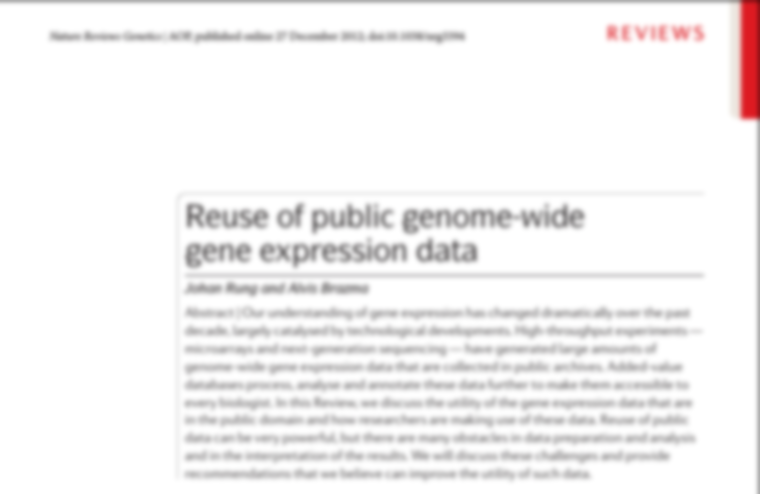
\includegraphics[width=0.8\columnwidth]{images/rung_brazma_2013_grey}};
      \node[align=center,red,font={\normalsize\bfseries}] at (image.center)
      {``The authors replicated two studies ‘in principle’\\ and six
        ‘partially’, whereas ten were not reproduced,\\ ...\\ The main
        reason for the lack of reproducibility \\ was the
        unavailability of all relevant data or metadata:''};
    \end{tikzpicture}
  }
  \only<3>{
    \begin{figure}
      
\includegraphics[width=0.8\columnwidth]{./images/hines_etal_2014}
    \end{figure}
  }
  \only<4> {
    \begin{tikzpicture}
      \node[anchor=south west,inner sep=0] (image) at (0,0) {
        
\includegraphics[width=0.8\columnwidth]{images/hines_etal_2014_grey}};
      \node[align=center,red,font={\normalsize\bfseries}] at
      (image.center) {``... our two laboratories quite reproducibly
        were unable\\ to replicate each other’s
        fluorescence-activated cell sorting \\ (FACS) profiles of
        primary breast cells.``};
    \end{tikzpicture}
  }
\end{frame}

\begin{frame}
  \frametitle{Towards standardization in the Neurosciences}
  \framesubtitle{Reproducing results is hindered by the lack of data}
  \begin{columns}
    \begin{column}{8cm}
      \begin{itemize}
      \item Improving the situation in the neurosciences was the reason
        to establish the INCF and the national nodes.
      \item The German Neuroinformatics Node (G-Node, at the Bernstein
        Center in Munich, established 2008) is one of the founding members.
      \item We (J.B. and J.G) have been involved right from the start.
      \item Were members of the INCF ``Standards for electrophysiology'' Task-force.
      \item Discussions therein were the starting point of the \nix{}
        development back in 2012.
      \end{itemize}
    \end{column}
    \begin{column}{4cm}
      
\includegraphics[width=0.8\columnwidth]{images/incf_logo.png}\\
      \vspace{5ex}
      
\includegraphics[width=0.8\columnwidth]{images/g-node_logo.png}
    \end{column}
  \end{columns}
\end{frame}

\section{NIX}
\begin{frame}
  \huge{\rot{Introduction to the \textit{NIX} Project}}
  \vspace{4ex}
  \begin{center}
    
\includegraphics[width=0.25\linewidth]{images/nix_logo.png}
  \end{center}
\end{frame}

\begin{frame}
  \frametitle{What is \nix{}?}
  \framesubtitle{Neuroscience Information exchange format}
  \noindent Design goals:
  \begin{itemize}
  \item Create a \textbf{generic} data model that can store a
    multitude of scientific data structures.
  \item Self-contained, i.e. all required information is stored in one container.
  \item We always want to be able to create a basic, yet completely labeled,
    plot of the data without asking someone else or addressing a
    different resource.
  \item Use as little entities as possible.
  \item Support embedded data annotations.
  \item Support standardization.
  \item Free, open-source, ...
  \end{itemize}
\end{frame}

\begin{frame}[fragile]
  \frametitle{Introduction to \nix{}}
  \framesubtitle{Which information needs to be stored?}

  \begin{center}
    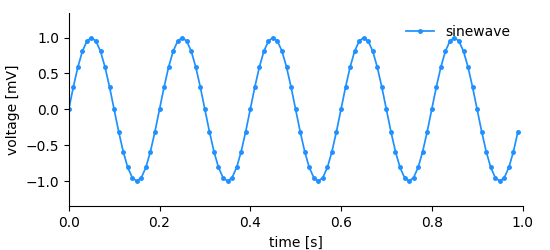
\includegraphics[width=0.7\columnwidth]{images/regular_sampled.png}
  \end{center}
  The plot shows voltage measurement taken at given times. We need to store:
  \begin{enumerate}
  \item the y-values (voltage measurements).
  \item the x-values (times at which the data was sampled).
  \item the label of the y-axis (voltage) and the unit (mV).
  \item the label of the x-axis (time) and the unit (s).
  \item the name of the trace for the legend.
  \end{enumerate}
\end{frame}


\begin{frame}[fragile]
  \frametitle{Introduction to \nix{}}
  \framesubtitle{Which information needs to be stored?}

  Some of the aforementioned information is ...
  \begin{itemize}
  \item directly related to the data.
  \item related to the dimensions of the dataset.
  \end{itemize}
  \pause
  \vspace{3ex}
  Accordingly, ...
  \begin{itemize}
  \item data-related information goes into the \dataarray{} entity.
  \item dimension-related info goes into ``Dimension descriptors''.
  \end{itemize}
\end{frame}


\begin{frame}
  \frametitle{Introduction to \nix{}}
  \framesubtitle{The \dataarray{}}
  \begin{columns}
    \begin{column}{5cm}
      \begin{itemize}
      \item The \dataarray{} is the core entity of the \nix{} data model.
      \item It stores the actual data.
      \item Plus a few more pieces of information.
      \end{itemize}
    \end{column}
    \begin{column}{6cm}
      \begin{table}[]
        \scriptsize
        \centering
        \captionsetup{labelformat=empty}
        \caption{DataArray}
        \begin{tabular}{|l|l|}
          \hline
          \rowcolor[HTML]{EFEFEF} 
          Field                   & Type             \\ \hline
          id                      & string           \\ \hline
          \textbf{name}           & string           \\ \hline
          type                    & string           \\ \hline
          definition              & string           \\ \hline
          \textbf{label}          & string           \\ \hline
          \textbf{unit}           & string           \\ \hline
          \textbf{data}           & n-d data         \\ \hline
          dtype                   & double, int, ... \\ \hline
          \textbf{dimensions}     & Dimension[]      \\ \hline
          sources[]               & Source []        \\ \hline
          metadata                & Section          \\ \hline
          polynom\_coefficients   & double []        \\ \hline
          expansion\_origin       & double           \\ \hline\hline
          createdAt               & datetime         \\ \hline
          updatedAt               & datetime         \\ \hline
        \end{tabular}
      \end{table}
      \normalsize
    \end{column}
  \end{columns}
\end{frame}


\begin{frame}
  \frametitle{Introduction to \nix{}}
  \framesubtitle{Dimension descriptors}
  Three (and a half) types of dimensions:
  \begin{enumerate}
  \item SampledDimension
  \item RangeDimension
  \item SetDimension
  \end{enumerate}
\end{frame}


\begin{frame}
  \frametitle{Introduction to \nix{}}
  \framesubtitle{Dimension Descriptors}
  \noindent \textbf{1: SampledDimension}
  \begin{center}
    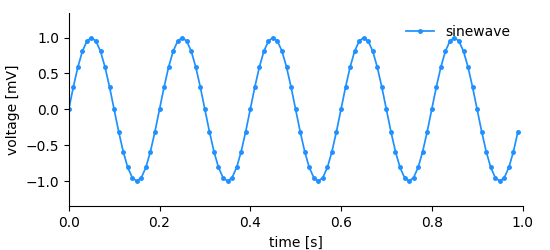
\includegraphics[width=0.85\linewidth]{images/regular_sampled.png}
  \end{center}
  \pause

  Used if data has been sampled in regular intervals. The descriptor
  stores the \textbf{label}, the \textbf{unit}, the \textbf{sampling
    interval} and the \textbf{offset} of the dimension (axis).
\end{frame}


\begin{frame}
  \frametitle{Introduction to \nix{}}
  \framesubtitle{Dimension Descriptors}
  \noindent \textbf{2: RangeDimension}
  \begin{center}
    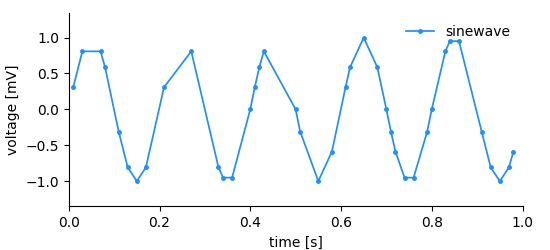
\includegraphics[width=0.85\linewidth]{images/irregular_sampled.png}
  \end{center}
  \pause
  Used if the data has been sampled in irregular intervals. The descriptor stores the
  \textbf{label}, the \textbf{unit}, and the \textbf{ticks} of the dimension (axis).
\end{frame}


\begin{frame}
  \frametitle{Introduction to \nix{}}
  \framesubtitle{Dimension Descriptors}
  \noindent \textbf{2b: AliasRangeDimension}
  \begin{center}
    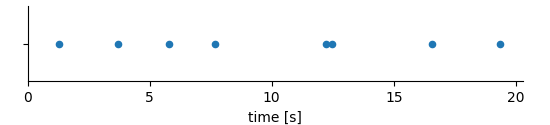
\includegraphics[width=0.85\linewidth]{images/alias_range.png}
  \end{center}
  \pause Used if the stored data are e.g the time-points of certain
  events.  The descriptor is basically a link to the stored data
  itself and can only be applied when the data is 1D.
\end{frame}


\begin{frame}
  \frametitle{Introduction to \nix{}}
  \framesubtitle{Dimension Descriptors}
  \noindent \textbf{3: SetDimension}

  \begin{center}
    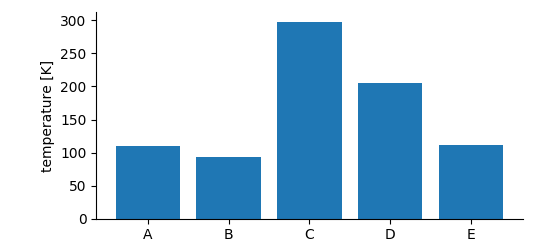
\includegraphics[width=0.85\linewidth]{images/set_dimension.png}
  \end{center}
  \pause

  Used if the axis represents categories that may not have a natural
  order.  The descriptor stores (optional) \textbf{label}s for each
  entry along the respective dimension.
\end{frame}

\begin{frame}
  \frametitle{Introduction to \nix{}}

  So far, we can ...
  \begin{enumerate}
    \item store n-dimensional data.
    \item provide information about type of values and the unit.
    \item describe the dimensions of the data.
  \end{enumerate}
  \pause
  But we want more:
  \begin{enumerate}
  \item Annotating/tagging data (regions or points).
  \item Add arbitrary metadata.
  \end{enumerate}
\end{frame}


\subsection{tagging}
\begin{frame}
  \frametitle{Introduction to \nix{}}
  \framesubtitle{Tagging things}
  We may record a system's response over time and want to note (tag)
  the time a stimulus was on.
  \begin{center}
    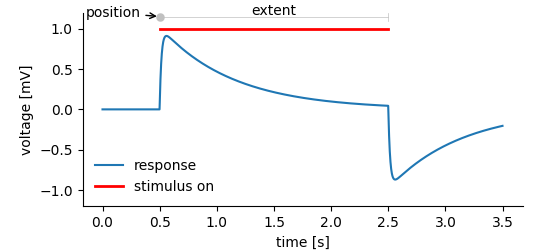
\includegraphics[width=0.85\columnwidth]{images/tag2.png}
  \end{center}
  \pause
  \textbf{Tag}s are used to annotate points or regions in
  the data stored in a \dataarray{}.

\end{frame}

\begin{frame}
  \frametitle{Introduction to \nix{}}
  \framesubtitle{Tagging things in 2D}
  The approach can be extended into n-D.

  \begin{center}
    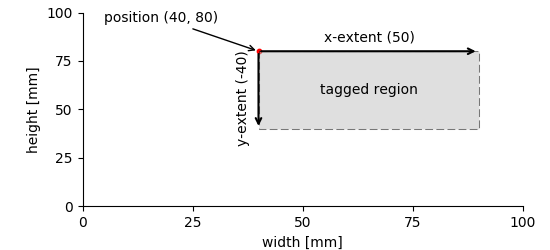
\includegraphics[width=0.85\columnwidth]{images/2d_tag.png}
  \end{center}
  \pause
  \textbf{position} and \textbf{extent} are now vectors of
  length n.
\end{frame}

\begin{frame}
  \frametitle{Introduction to \nix{}}
  \framesubtitle{Tagging many things at once}
  \begin{center}
    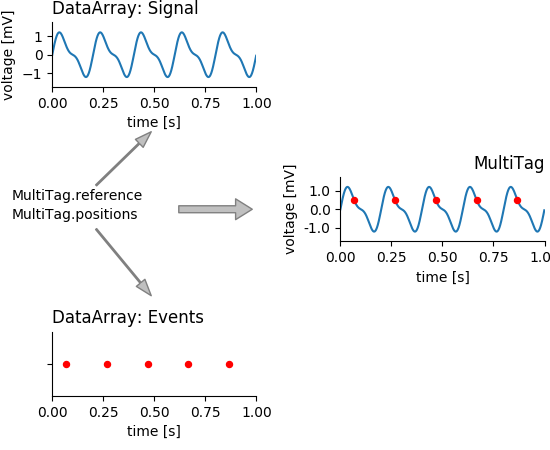
\includegraphics[width=0.775\columnwidth]{images/mtag_concept.png}
  \end{center}
  \pause

  A \textbf{MultiTag} entity is used to bind two (or more)
  \dataarray{}s.
\end{frame}

\begin{frame}
  \frametitle{Introduction to \nix{}}
  \only<1> {
    \framesubtitle{Tagging multiple regions in 2D}
    \begin{center}
      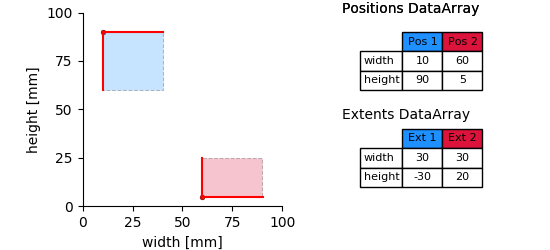
\includegraphics[width=0.85\columnwidth]{images/2d_mtag.png}
    \end{center}
  }
  \only<2> {
    \framesubtitle{Tagging multiple hyperslaps}
    \begin{center}
      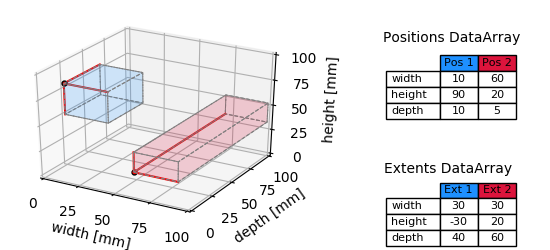
\includegraphics[width=0.85\columnwidth]{images/3d_mtag.png}
    \end{center}
  }
\end{frame}


\begin{frame}
  \frametitle{Introduction to \nix{}}
  \framesubtitle{Tagging}
  \begin{columns}
    \begin{column}{5cm}
      Tags act as a hub that ...
      \begin{itemize}
      \item links \dataarray{}s.
      \item tags points or regions in n-D.
      \end{itemize}
      But we need more:
      \begin{itemize}
      \item A way to give some more meaning to the tagged regions.
      \item Add metadata.
      \end{itemize}
    \end{column}
    \begin{column}{6cm}
       \begin{table}[]
        \scriptsize
        \centering
        \captionsetup{labelformat=empty}
        \caption{Tag}
        \begin{tabular}{|l|l|}
          \hline
          \rowcolor[HTML]{EFEFEF} 
          Field                   & Type             \\ \hline
          id                      & string           \\ \hline
          name                    & string           \\ \hline
          type                    & string           \\ \hline
          definition              & string           \\ \hline
          \textbf{position}       & double []        \\ \hline
          \textbf{extent}         & double []        \\ \hline
          units                   & string []        \\ \hline
          \textbf{references}     & DataArray []     \\ \hline
          features                & Feature []       \\ \hline
          sources                 & Source []        \\ \hline
          metadata                & Section          \\ \hline \hline
          createdAt               & datetime         \\ \hline
          updatedAt               & datetime         \\ \hline
        \end{tabular}
      \end{table}
      \normalsize
    \end{column}
  \end{columns}
\end{frame}

\subsection{features}

\begin{frame}
  \frametitle{Introduction to \nix{}}
  \framesubtitle{Features}
  Feature entities are used to attach some more information to tagged regions.

  For example:
  \begin{itemize}
  \item Each tagged region has characteristics that need to be stored
    (e.g. the $\frac{\Delta f}{f}$ ratio in a region of interest).
  \item In each tagged regions a stimulus of a certain intensity was used.
  \item The power spectrum of the neuronal response in the tagged
    regions have been estimated.
  \item ...
  \end{itemize}
  \pause{}
  \begin{table}[]
    \scriptsize
    \centering
    \captionsetup{labelformat=empty}
    \caption{Feature}
    \begin{tabular}{|l|l|}
      \hline
      \rowcolor[HTML]{EFEFEF} 
      Field                   & Type             \\ \hline
      id                      & string           \\ \hline
      link\_type              & LinkType         \\ \hline
      data                    & DataArray        \\ \hline
    \end{tabular}
  \end{table}
  \normalsize
\end{frame}

\begin{frame}
  \frametitle{Introduction to \nix{}}
  \framesubtitle{Features}
  Depending on the type of feature there are three ways how the
  features of a tag should be interpreted (by the library or the
  user).
  \pause{}
  \begin{enumerate}
  \item \textbf{Indexed}: For each position of the Tag, there is an entry along
    the first dimension of the data which contains the feature.
  \item \textbf{Tagged}: positions and extents of the Tag also apply
    to the feature.
  \item \textbf{Untagged}: all the data stored in the feature relates
    to the Tag irrespective of positions and extents.
  \end{enumerate}
\end{frame}

\subsection{Metadata}
\begin{frame}
  \frametitle{Introduction to \nix{}}
  \framesubtitle{Adding arbitrary metadata}
  \begin{columns}
    \begin{column}{6.5cm}
      \begin{enumerate}
      \item Many entities of the \nix{} data model allow adding more metadata.
      \item We use a simple tree-like structure of \textbf{Sections},
        \textbf{Properties} and \textbf{Values} for storing these.
      \end{enumerate}
    \end{column}
    \begin{column}{5cm}
      \begin{center}
        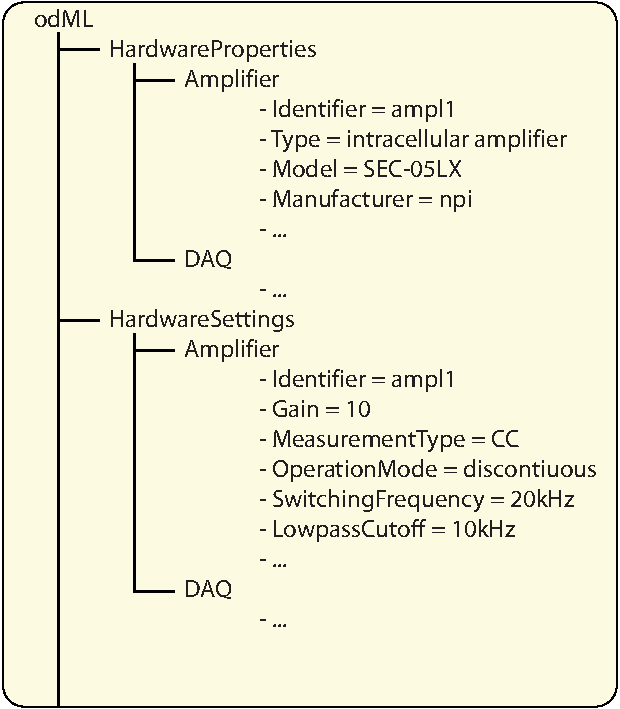
\includegraphics[width=\columnwidth]{images/metadata.pdf}
      \end{center}
    \end{column}
  \end{columns}
\end{frame}

\begin{frame}
  \frametitle{Introduction to \nix{}}
  \framesubtitle{NIX Data model}
  \begin{center}
    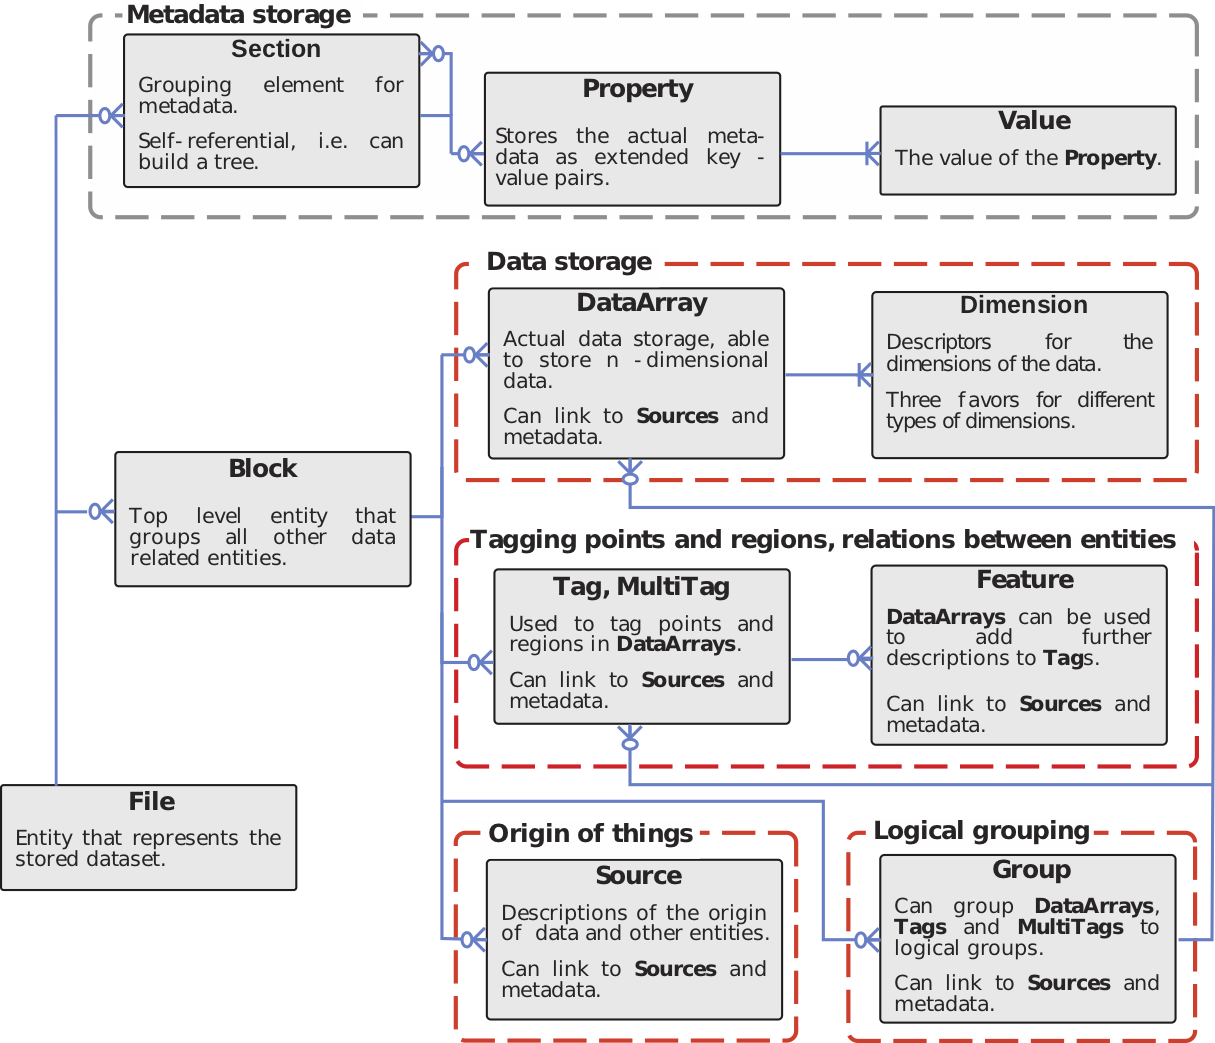
\includegraphics[width=0.85\linewidth]{images/data_model_brief.png}
  \end{center}
\end{frame}

\subsection{ecosystem}

\begin{frame}[fragile]
  \frametitle{Introduction to \nix{}}
  \framesubtitle{API design}
  \begin{center}
    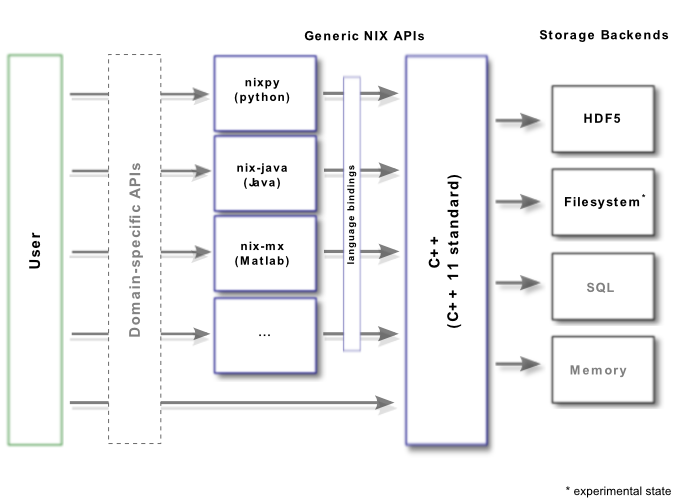
\includegraphics[width=0.95\linewidth]{images/api_design.png}
  \end{center}
\end{frame}


\begin{frame}[fragile]
  \frametitle{Introduction to \nix{}}
  \framesubtitle{\nix{} ecosystem}

  \begin{enumerate}
  \item NIX C++ library: \\\url{https://github.com/g-node/nix}
  \item nixpy python library: \\\url{https://github.com/g-node/nixpy}
  \item nix-java java library: \\\url{https://github.com/g-node/nix-java}
  \item nix-mx matlab library: \\\url{https://github.com/g-node/nix-mx}
    \vspace{1cm}
  \item storage backend for the NEO object model \\\url{neuralensemble.org}
  \item nixview: Viewer for nix files \\\url{https://github.com/bendalab/nixview}
  \end{enumerate}
\end{frame}

\begin{frame}
 \huge{\rot{phew ...}}
\end{frame}

%%%%%%%%%%%%%%%%%%%%%%%%%%%%%%%%%%%%%%%%%%%%%%%%%%%%%%%%%%%%%%%%%
%%%%%%%%%%%%%%%%%%%%%%%%%%%%%%%%%%%%%%%%%%%%%%%%%%%%%%%%%%%%%%%%%

\section{Integration in RELACS}

\begin{frame}
  \huge{\rot{Integration of \nix{} in RELACS}}
  \vspace{4ex}
   \begin{center}
    
\includegraphics[width=0.25\columnwidth]{images/relacstux.png}
  \end{center}
\end{frame}

\begin{frame}
  \frametitle{Integration of \nix{} in RELACS}
  \framesubtitle{RELACS overview}
  \only<1> {
  \begin{center}
    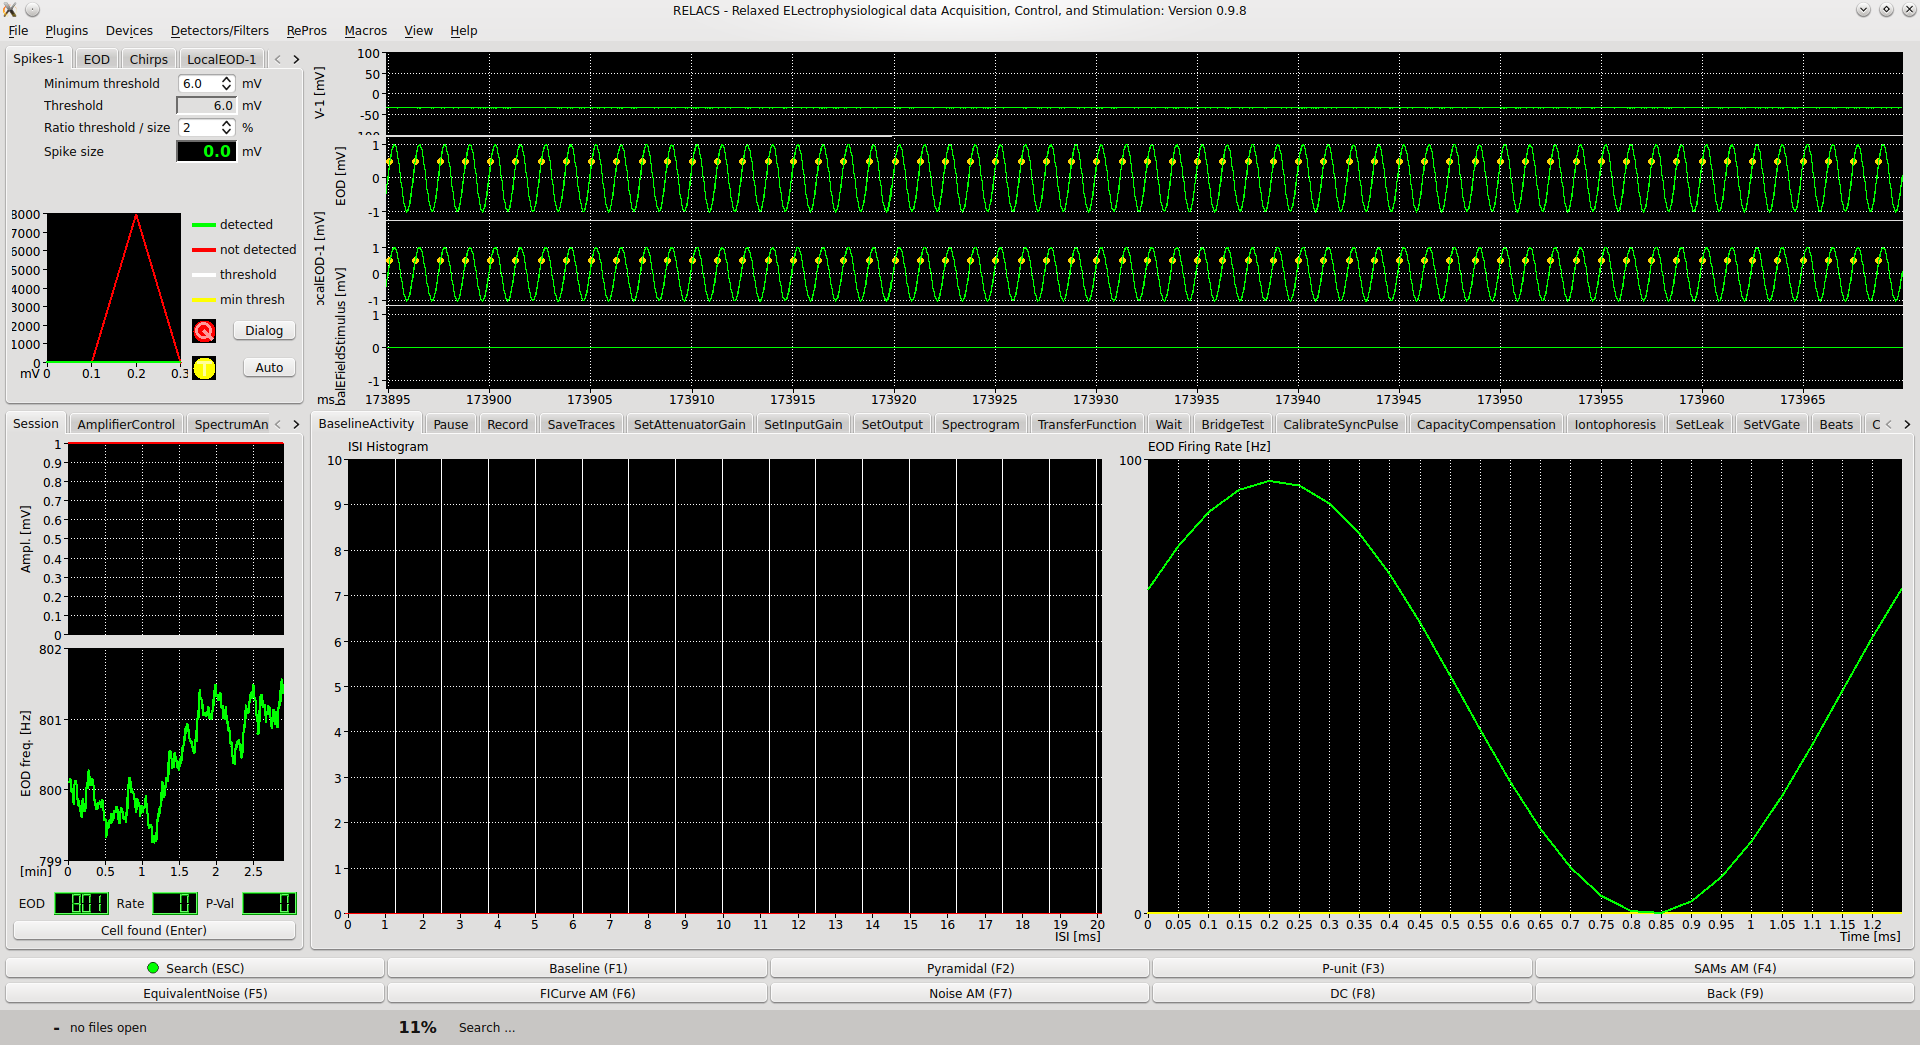
\includegraphics[width=\columnwidth]{images/relacs_ephys}
  \end{center}
  }\only <2> {
    \begin{center}
      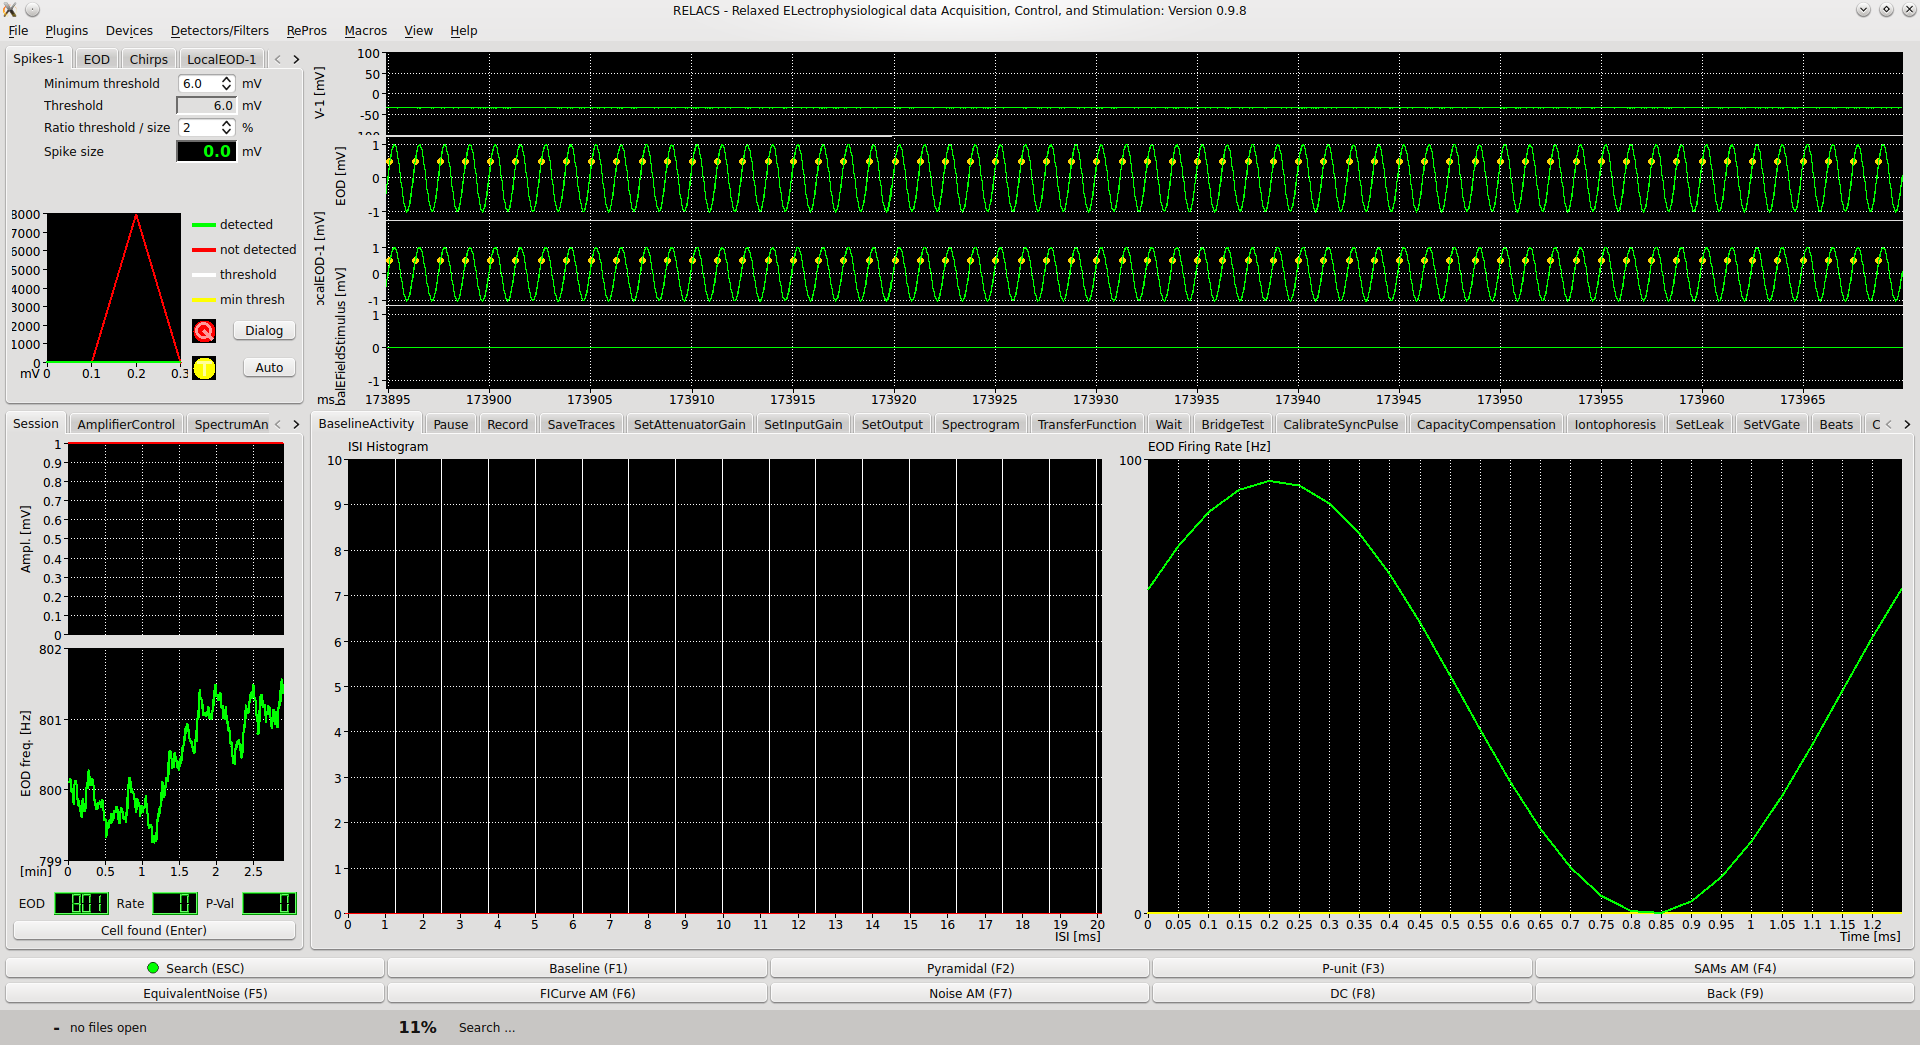
\includegraphics[width=0.45\columnwidth]{images/relacs_ephys}
    \end{center}
    Storing various datasets.
    \begin{enumerate}
    \item The membrane voltage (V-1).
    \item The fish's electric organ discharge (EOD), global measurement.
    \item The local measurement of the EOD (LocalEOD-1).
    \item The stimulus put into the tank (GlobalEFieldStimulus).
    \item The times of detected spikes (Spikes-1).
    \item Sometimes the times of EOD discharges and detected chirps.
    \end{enumerate}
  }
\end{frame}


\begin{frame}
  \frametitle{Integration of \nix{} in RELACS}
  \framesubtitle{RELACS overview}
  \begin{enumerate}
  \item Relacs acquires data and controls the stimulus output.
  \item knows a lot of metadata.
  \end{enumerate}
  \begin{columns}
    \begin{column}{6cm}
      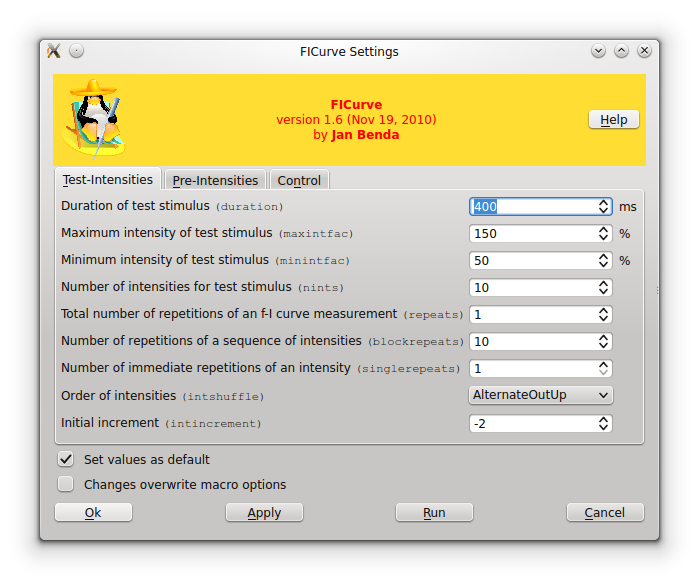
\includegraphics[width=\columnwidth]{images/relacs_ephys_options}
    \end{column}
    \begin{column}{6cm}
      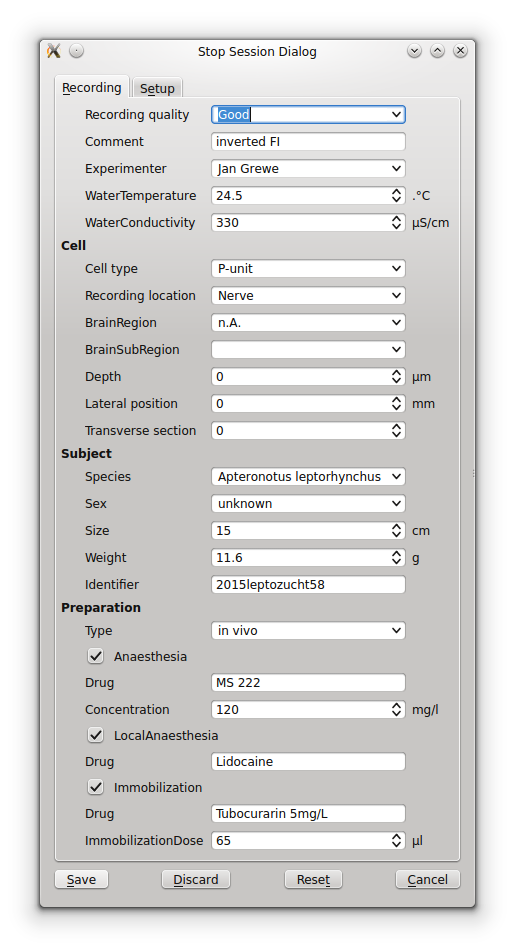
\includegraphics[width=0.7\columnwidth]{images/relacs_ephys_mdata}
    \end{column}
  \end{columns}
\end{frame}


\begin{frame}
  \frametitle{Integration of \nix{} in RELACS}
  \framesubtitle{A recording session in RELACS}

  Once we press ``Enter'', we may run some macros that in turn run
  research protocols (repros) with various parameter sets and put out
  certain stimuli.

  \begin{center}
    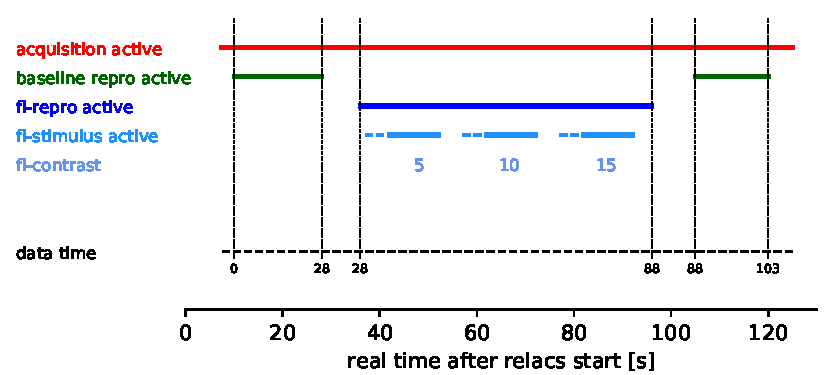
\includegraphics[width=0.9\columnwidth]{images/relacs_timeline}
  \end{center}

  Data is not always dumped to file. The ``data time'' does not
  necessarily match the real time.
\end{frame}


\begin{frame}
  \frametitle{Integration of \nix{} in RELACS}
  \framesubtitle{Representing RELACS data in \nix{}}
  \begin{center}
    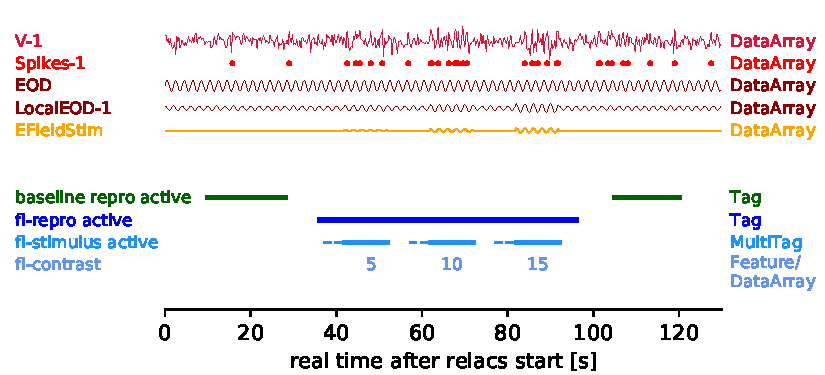
\includegraphics[width=0.9\columnwidth]{images/relacs_tagging}
  \end{center}
\end{frame}

\begin{frame}
  \frametitle{Integration of \nix{} in RELACS}
  \framesubtitle{Representing RELACS data in \nix{}}
  \begin{itemize}
  \item For each recording (pressing of enter) we create a new dataset.
  \item In each dataset we find only a single \textbf{Block} that
    contains all data.
  \item We always have as many \dataarray{}s as there are input channels
    and event channels (from Filters and Detectors).
  \item For each run of a repro, there will be one \textbf{Tag}
    (usually named according to the repro name with a number suffix).
  \item For each repro we have a \textbf{MultiTag} to store the
    stimulus-on segments.
  \item Repro settings go to the metadata into a \textbf{Section} that
    has the same name as the repro \textbf{Tag}.
  \item If the stimulus settings change, a new \textbf{MultiTag} will be created.
  \item Except if the chaning setting is set as ``mutable'', then it
    will become a \textbf{Feature} of the respective
    \textbf{MultiTag}.
  \end{itemize}
\end{frame}
%%%%%%%%%%%%%%%%%%%%%%%%%%%%%%%%%%%%%%%%%%%%%%%%%%%%%%%%%%%%%%%%%
%%%%%%%%%%%%%%%%%%%%%%%%%%%%%%%%%%%%%%%%%%%%%%%%%%%%%%%%%%%%%%%%%
\section{Working with the nix files}

\begin{frame}
  \huge{\rot{Working with relacs-flavored nix-files}}\\
  \begin{center}
  \end{center}
\end{frame}

\begin{frame}[fragile]
  \frametitle{Working with relacs-flavored \nix{} files}
  \framesubtitle{Basic structure of the file}

  Any \nix{} file has two top-level ``folders'' blocks, and
  sections. For data and metadata, respectively. There will be only one
  \textbf{Block} that represents the recording session.

  \inputminted[bgcolor=lstbg, linenos=false, fontsize=\footnotesize]{bash}{code/open_file.py}
\end{frame}

\begin{frame}[fragile]
  \frametitle{Working with relacs-flavored \nix{} files}
  \framesubtitle{Accessing DataArrays}

  \inputminted[bgcolor=lstbg, linenos=false, fontsize=\footnotesize, firstline=4]{bash}{code/playground1.py}
\end{frame}


\begin{frame}[fragile]
  \frametitle{Working with relacs-flavored \nix{} files}
  \framesubtitle{Accessing DataArrays}

  \inputminted[bgcolor=lstbg, linenos=false, fontsize=\scriptsize, firstline=9, lastline=27]{bash}{code/playground2.py}
\end{frame}


\begin{frame}[fragile]
  \frametitle{Working with relacs-flavored \nix{} files}
  \framesubtitle{What else?}
  \begin{enumerate}
  \item With the use of the nix-files we achieve a (more or less)
    common data storage.
  \item Data and metadata reside within the same container.
  \item We can hope for a common toolbox for accessing the recorded
    data.
  \end{enumerate}

  \begin{itemize}
  \item More examples required?
  \item How can we improve the storing of data?
  \item What functionality should be provided by the nix-libraries?
  \end{itemize}
\end{frame}


\section{Summary} 
\begin{frame}
  \frametitle{People}
  Quite a few people are, or have been, involved in the development:

  \begin{columns}
    \begin{column}{5cm}
      \begin{itemize}
      \item[] Jan Benda
      \item[] Christian Garbers
      \item[] \textbf{Jan Grewe}
      \item[] \textbf{Christian Kellner}
      \item[] \textbf{Achilleas Koutsou}
      \item[] Balint Morvai
      \item[] \textbf{Michael Sonntag}
      \item[] \textbf{Adrain Stoewer}
      \item[] Andrey Sobolev
      \item[] \textbf{Thomas Wachtler}
      \end{itemize}
    \end{column}
    \begin{column}{5cm}
      \begin{itemize}
      \item[] Alexander Ott
      \item[] Lorand Madai
      \item[] Fabian Woltermann
      \item[] @matham
      \item[] @sudoankit
      \item[] @Prabhanit
      \item[] @digaru19
      \item[] @sOnskar
      \item[] @saurabhiiit
      \item[] @sujithvm
      \end{itemize}
    \end{column}
  \end{columns}
\end{frame}


\begin{frame}
   \begin{center}
   
\includegraphics[width=0.95\columnwidth]{images/phd092506s.png}
  \end{center}
\end{frame}


\end{document}
